\documentclass[12pt,twoside]{article}
%%%%%%%%%%%%%%%%%%%%%%%%%%%%%%%%%%%%%%%%%%%%%%%%%%%%%%%%%%%%%
% Meta informations:
\newcommand{\trauthor}{Soubarna Banik}
\newcommand{\trtype}{Project Report} %{Seminararbeit} %{Proseminararbeit}
\newcommand{\trcourse}{Independent Study}
\newcommand{\trtitle}{Road Detection Using Hyperspectral Image}
\newcommand{\trmatrikelnummer}{6640587}
\newcommand{\tremail}{4banik@informatik.uni-hamburg.de}
\newcommand{\trarbeitsbereich}{Cognitive Systems Laboratory, KOGS}
\newcommand{\trdate}{31.12.2016}

%%%%%%%%%%%%%%%%%%%%%%%%%%%%%%%%%%%%%%%%%%%%%%%%%%%%%%%%%%%%%
% Languages:

% Falls die Ausarbeitung in Deutsch erfolgt:
% \usepackage[german]{babel}
% \usepackage[T1]{fontenc}
% \usepackage[latin1]{inputenc}
% \usepackage[latin9]{inputenc}	 				
% \selectlanguage{german}

% If the thesis is written in English:
\usepackage[english]{babel} 						
\selectlanguage{english}

%%%%%%%%%%%%%%%%%%%%%%%%%%%%%%%%%%%%%%%%%%%%%%%%%%%%%%%%%%%%%
% Bind packages:
\usepackage{acronym}                    % Acronyms
\usepackage{algorithmic}								% Algorithms and Pseudocode					
\usepackage{algorithm2e}
\usepackage{amsfonts}                   % AMS Math Packet (Fonts)
\usepackage{amsmath}                    % AMS Math Packet
\usepackage{amssymb}                    % Additional mathematical symbols
\usepackage{amsthm}
\usepackage{booktabs}                   % Nicer tables
\usepackage[font=small,labelfont=bf]{caption} % Numbered captions for figures
\usepackage{color}                      % Enables defining of colors via \definecolor
\definecolor{uhhRed}{RGB}{254,0,0}		  % Official Uni Hamburg Red
\definecolor{uhhGrey}{RGB}{122,122,120} % Official Uni Hamburg Grey
\usepackage{fancybox}                   % Gleichungen einrahmen
\usepackage{fancyhdr}										% Packet for nicer headers
%\usepackage{fancyheadings}             % Nicer numbering of headlines

%\usepackage[outer=3.35cm]{geometry} 	  % Type area (size, margins...) !!!Release version
%\usepackage[outer=2.5cm]{geometry} 		% Type area (size, margins...) !!!Print version
%\usepackage{geometry} 									% Type area (size, margins...) !!!Proofread version
\usepackage[outer=3.15cm]{geometry} 	  % Type area (size, margins...) !!!Draft version
\geometry{a4paper,body={5.8in,9in}}

\usepackage{graphicx}                   % Inclusion of graphics
\usepackage{wrapfig}

%\usepackage{latexsym}                  % Special symbols
\usepackage{longtable}									% Allow tables over several parges
\usepackage{listings}                   % Nicer source code listings
\usepackage{multicol}										% Content of a table over several columns
\usepackage{multirow}										% Content of a table over several rows
\usepackage{rotating}										% Alows to rotate text and objects
\usepackage[hang]{subfigure}            % Allows to use multiple (partial) figures in a fig
%\usepackage[font=footnotesize,labelfont=rm]{subfig}	% Pictures in a floating environment
\usepackage{tabularx}										% Tables with fixed width but variable rows
\usepackage{url,xspace,boxedminipage}   % Accurate display of URLs
%%%%%%%%%%%%%%%%%%%%%%%%%%%%%%%%%%%%%%%%%%%%%%%%%%%%%%%%%%%%%
% Configurationen:

\hyphenation{whe-ther} 									% Manually use: "\-" in a word: Staats\-ver\-trag

%\lstloadlanguages{C}                   % Set the default language for listings
\DeclareGraphicsExtensions{.pdf,.svg,.jpg,.png,.eps} % first try pdf, then eps, png and jpg
\graphicspath{{./src/}} 								% Path to a folder where all pictures are located
\pagestyle{fancy} 											% Use nicer header and footer

% Redefine the environments for floating objects:
\setcounter{topnumber}{3}
\setcounter{bottomnumber}{2}
\setcounter{totalnumber}{4}
\renewcommand{\topfraction}{0.9} 			  %Standard: 0.7
\renewcommand{\bottomfraction}{0.5}		  %Standard: 0.3
\renewcommand{\textfraction}{0.1}		  	%Standard: 0.2
\renewcommand{\floatpagefraction}{0.8} 	%Standard: 0.5

% Tables with a nicer padding:
\renewcommand{\arraystretch}{1.2}

%%%%%%%%%%%%%%%%%%%%%%%%%%%%
% Additional 'theorem' and 'definition' blocks:
\theoremstyle{plain}
\newtheorem{theorem}{Theorem}[section]
%\newtheorem{theorem}{Satz}[section]		% Wenn in Deutsch geschrieben wird.
\newtheorem{axiom}{Axiom}[section] 	
%\newtheorem{axiom}{Fakt}[chapter]			% Wenn in Deutsch geschrieben wird.
%Usage:%\begin{axiom}[optional description]%Main part%\end{fakt}

\theoremstyle{definition}
\newtheorem{definition}{Definition}[section]

%Additional types of axioms:
\newtheorem{lemma}[axiom]{Lemma}
\newtheorem{observation}[axiom]{Observation}

%Additional types of definitions:
\theoremstyle{remark}
%\newtheorem{remark}[definition]{Bemerkung} % Wenn in Deutsch geschrieben wird.
\newtheorem{remark}[definition]{Remark} 

%%%%%%%%%%%%%%%%%%%%%%%%%%%%
% Provides TODOs within the margin:
\newcommand{\TODO}[1]{\marginpar{\emph{\small{{\bf TODO: } #1}}}}
\newcommand{\forceindent}{\leavevmode{\parindent=2em\indent}}
%%%%%%%%%%%%%%%%%%%%%%%%%%%%
% Abbreviations and mathematical symbols
\newcommand{\modd}{\text{ mod }}
\newcommand{\RS}{\mathbb{R}}
\newcommand{\NS}{\mathbb{N}}
\newcommand{\ZS}{\mathbb{Z}}
\newcommand{\dnormal}{\mathit{N}}
\newcommand{\duniform}{\mathit{U}}

\newcommand{\erdos}{Erd\H{o}s}
\newcommand{\renyi}{-R\'{e}nyi}
%%%%%%%%%%%%%%%%%%%%%%%%%%%%%%%%%%%%%%%%%%%%%%%%%%%%%%%%%%%%%
% Document:
\begin{document}
\renewcommand{\headheight}{14.5pt}

\fancyhead{}
\fancyhead[LE]{ \slshape \trauthor}
\fancyhead[LO]{}
\fancyhead[RE]{}
\fancyhead[RO]{ \slshape \trtitle}

%%%%%%%%%%%%%%%%%%%%%%%%%%%%
% Cover Header:
\begin{titlepage}
	\begin{flushleft}
		Universit\"at Hamburg\\
		Department Informatik\\
		\trarbeitsbereich\\
	\end{flushleft}
	\vspace{3.5cm}
	\begin{center}
		\huge \trtitle\\
	\end{center}
	\vspace{3.5cm}
	\begin{center}
		\normalsize\trtype\\
		[0.2cm]
		\Large\trcourse\\
		[1.5cm]
		\Large \trauthor\\
		[0.2cm]
		\normalsize Matr.Nr. \trmatrikelnummer\\
		[0.2cm]
		\normalsize\tremail\\
		[1.5cm]
		\Large \trdate
	\end{center}
	\vfill
\end{titlepage}

	%backsite of cover sheet is empty!
\thispagestyle{empty}
\hspace{1cm}
\newpage

%%%%%%%%%%%%%%%%%%%%%%%%%%%%
% Abstract:

% Abstract gives a brief summary of the main points of a paper:
\section*{Abstract}

% Lists:
\setcounter{tocdepth}{2} 					% depth of the table of contents (for Seminars 2 is recommented)
\tableofcontents
\pagenumbering{arabic}
\clearpage

%%%%%%%%%%%%%%%%%%%%%%%%%%%%
% Content:

% the actual content, usually separated over a number of sections
% each section is assigned a label, in order to be able to put a
% crossreference to it

\section{Introduction}
\label{sec:introduction}
Advancements in hyperspectral imaging technologies have opened up an entirely new way of looking at our planet, and have added considerably to our knowledge about it. Hyperspectral spectrometers capture high resolution images consisting usually of more than a hundred bands/channels. Remotely sensed RGB or multispectral data often do not provide sufficient information for differentiating similar looking materials. Also the task is more complex as the images are captured from such long distance. The unique continuous reflectance spectra of different materials has made it possible to identify target materials from remotely sensed hyperspectral images. Its benefit can be reaped across a variety of applications, such as vegetation identification, agricultural monitoring, atmospheric and ocean characteristics study, mineral exploration, environmental monitoring etc. Another key application of remote sensing is urban monitoring. As per the World Health Organisation (WHO) the urban population in 2014 accounted for 54\% of  the total global population \footnote{\url{http://www.who.int/gho/urban_health/situation_trends/urban_population_growth_text/en/}}. This rapid growth needs to be monitored to ensure urban planning, future development and sustainable growth. 
Road network identification is an important aspect of urban monitoring as it can be considered as a measure of urbanization. It also provides significant information for planning transportation. Most of the current road mapping algorithms require manual intervention, which are tedious and time-consuming processes.\\
However, with hundreds of bands, hyperspectral images suffer from the problem of high data dimensionality. Though state of the art machine learning algorithms can overcome this problem, it is not always possible to acquire enough hyperspectral data samples as these images are costly. Also, the measurements of the individual pixels are often prone to noise and intra-class variability of spectra \cite{thompson2010superpixel}. Superpixel segmentation act as a solution to both problems of high data dimensionality and noise. The term "superpixel" was introduced by Ren and Malik in \cite{ren2003learning} to indicate a group of pixels that are local and coherent in features. By representing a set of pixels with a single superpixel, the data redundancy in images reduces considerably. It is also beneficial to run optimization algorithms on superpixels rather than at pixel level, which is computationally expensive, and at times infeasible due to large number of pixels in high resolution images. Classification of hyperspectral data at superpixel level, hence, reduces the computational complexity, as well as reduces the effect of noise.\\
In this paper, a fully automatic superpixel-based road detection algorithm is proposed. The paper is organized as follows - section \ref{sec:relatedwork} gives a description of the existing road extraction models. Hyperspectral image and its characteristics are described in section \ref{sec:HypTheo}. Section \ref{sec:model} depicts the proposed superpixel based road extraction method and section \ref{sec:experiment} evaluates the experimental results. Finally a conclusion is reached in section \ref{sec:concl}.

\section{Related Work}
\label{sec:relatedwork}
Plethora of work has been done in road detection, road network extraction, road centerline determination etc. since the last three decades. These work are broadly categorised by Poullis et al. in \cite{Poullis2010} into three categories - pixel based, region based and knowledge-based techniques. The pixel-based methods operate directly on the pixels. Most of the initial work on road detection is pixel based. A few examples of the recent pixel based work are road network detection from multispectral imagery by Zhang et al. \cite{Zhang2006}, a vision-based system for automatic road detection by Poullis et al. \cite{Poullis2010} etc. The region-based methods segment the images into regions, and operate on the regions in stead of the individual pixels, thereby reducing computation cost. Some of the region based approaches include a higher order CRF(conditional random field) model based on superpixels \cite{Wegner2013}, a graph based road tracking system \cite{Seppke2016} and a road centerline extraction model using multiscale segmentation and tensor voting \cite{Cheng}. The knowledge-based methods take some higher level information into consideration - such as the geometric and radiometric properties of road, or some contextual information etc. \\Road detection systems can also be grouped into semi-automatic and fully automatic approaches. Semi-automatic approaches relies on initial seed points for tracking or requires some intervention by a human operator. For example, the previously mentioned method in \cite{Seppke2016} relies on initial seed points. On the other hand the fully automatic approaches need no such human intervention. In addition to this there are supervised and unsupervised road classification methods. However, the supervised approaches need labelled data and as the ground truth determination is a very tedious process, it's availability is scarce. Unsupervised fully automatic approaches overcome these hurdles, however novel validation techniques are required in order to avoid dependency on labelled ground truth data.\\Many of the road detection approaches utilize different geometric properties of road to improve the models' performance. Two such common properties are the linearity and large area of road segments. For example, Miao et al. uses \textit{linear feature index} (LFI), a ratio of the length and width of the minimum bounding box of a segment in \cite{Miao2013}. Cheng et al. uses three different shape features in \cite{Cheng} - \textit{shape index} (SI), a ratio of perimeter and area of a segment, \textit{aspect ratio} (AR), ratio of the length and width of the bounding box of segments, and \textit{elliptical LFI}, where the ratio is computed for the bounding ellipse in stead of the bounding box. Though Cheng et al. has argued against the normal LFI, the aspect ratio feature used by them is similar to the LFI feature. Few other properties that have been utilised in research are the ratio of segment area and bounding box area, circularity and convexity a segment etc. Looking at the various pros and cons of the above mentioned approaches, a region based unsupervised approach for road detection is proposed in this paper. The proposed model utilizes the hyperspectral and geometric properties of road for detection.

\section{Hyperspectral Data Theory}
\label{sec:HypTheo}
Before hyperspectral data, multispectral data provided the opportunity to analyze target materials in electromagnetic (EM) wavebands other than the widely used visible (red, green and blue) wavebands. A spectrometer measures the reflectance of the materials in each waveband. Reflectance is the percentage of radiation incident on a material that is reflected by the material. A reflectance spectrum shows the reflectance of a material measured across a range of wavelengths \cite{shippert2003introduction}. The Landsat Thematic Mapper and SPOT XS satellite sensors produce multispectral images. The number of bands used to produce multispectral images are few (7 and 4 respectively) and relatively broad. For example, the SPOT XS multispectral images have bandwidth in the range of $10 \mu m$. On the other hand, hyperspectral spectrometers acquire images in much narrower bands ($10-20nm$). The narrower and contiguous bands of hyperspectral images helps in creating continuous spectrum which uniquely identifies each material. Each material responds uniquely to the incident radiations - in some wavelengths, its reflectance is high, whereas some other material absorbs highly in the same wavelengths.\\
\begin{wrapfigure}{l}{0.55\textwidth}
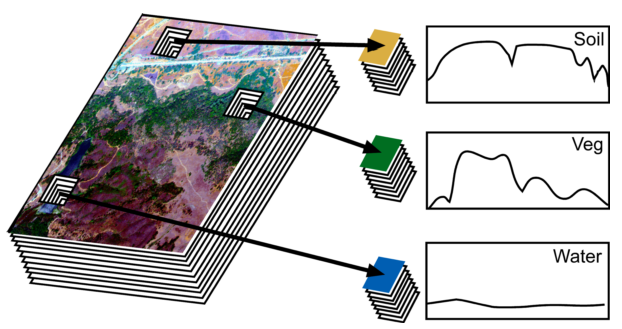
\includegraphics[width=0.55\textwidth]{src/Hyperspectral_cube.png}
\caption{Hyperspectral cube and a plot of reflectance spectrum of three pixels \cite{shippert2003introduction}}
\label{fig:hyp_cube}
\end{wrapfigure}
\forceindent \textit{Hyperspectral Cube:} A hyperspectral image is usually represented as a cube, containing two spatial dimensions and one spectral dimension. The spectral dimension consists of many narrow, adjacent wavelength bands. Figure \ref{fig:hyp_cube} shows a sample hyperspectral cube and the reflectance spectra of three sample pixels against the EM wavelengths. It can be seen, the spectral signature is different for the three different materials - soil, vegetation and water and thus, these materials can be identified by their reflectance spectra.
\begin{figure}[hbtp]
\centering
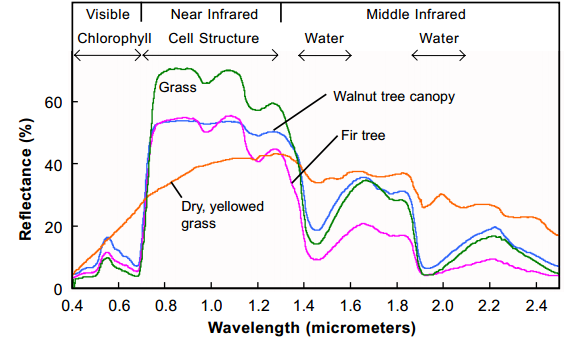
\includegraphics[width=0.75\textwidth]{src/plant_spectra.png}
\caption{Reflectance spectra of different types of plants. Different plant components contribute to different portions of the spectra \cite{smith2012} }
\label{fig:plant_spec}
\end{figure}
Even individual material belonging to the same class differs in their spectra. For example, different plant species have different spectral signature due to varied leaf structure, chlorophyll and water contents etc. As seen in Figure \ref{fig:plant_spec}, the spectral signatures are different for grass, trees and even for dry yellowed grass, though they belong to the same class, vegetation. Different components of plants contribute to different portions of the spectra.\\
\forceindent \textit{Spectral Libraries and Classification:} There are several spectral libraries available that consists of collections of reflectance spectra of natural as well as composite materials of known compositions. Besides, different datasets are also accompanied by their own spectral libraries, containing the spectra for the materials in the corresponding field site.  ASTER spectral library by NASA \cite{baldridge2009aster} and USGS spectral library by the United States Geological Survey Spectroscopy Lab \cite{clark1993us} etc. are some of the well-known public spectral libraries. Spectral libraries are used to classify hyperspectral images. The reflectance spectra of hyperspectral pixels are compared with the spectral library to identify the nearest matching constituent material.\\
\forceindent \textit{Spectral Unmixing:} Often, due to the limited spatial resolution of hyperspectral image, several materials contribute towards the spectrum of a pixel and it becomes hard to classify a pixel from its reflectance spectrum. In this scenario, a method called spectral unmixing is applied to quantify the proportion of each contributing materials in a pixel. Spectral unmixing algorithms generate an abundance map, which reports the percentage of all the pure surface materials, also called endmembers, for every pixel. Spectral unmixing algorithms can be both linear and non-linear. The linear algorithms are applied in case of  checkerboard mixture of materials in a pixel, where the materials lie side by side. In such mixture, incident rays reflect only once, from the surface, yielding a linear relationship between the fractional abundance and the reflected spectra \cite{keshava2000algorithm}. In case of a random mixture of materials, the incident rays are reflected multiple times by the materials, thereby producing a non-linear relationship between the final reflected spectra and the abundance fractions. This is depicted in Figure \ref{fig:unmix}.
\begin{figure}[hbtp]
\centering
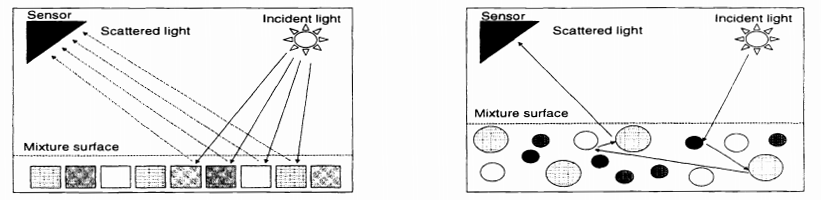
\includegraphics[width=0.95\textwidth]{src/spectral_unmixing.png}
\caption{Spectral unmixing: linear mixing from a checkerboard mixture having a single reflection (left), non-linear mixing from an intimate mixture having multiple reflections (right) \cite{keshava2000algorithm}}
\label{fig:unmix}
\end{figure}

\section{Road Detection using Hyperspectral Data}
\label{sec:model}
In this section, the proposed superpixel based road detection method is described. The method can be divided into two stages - an initial superpixel segmentation, followed by a classification stage. 

\subsection{Image Data}
Berlin-Urban-Gradient dataset is a ready-to-use multi-scale imaging spectrometer dataset prepared by GFZ German Research Center for Geosciences \cite{okujeni2016berlinurbangradient}. The dataset contains two HyMap scenes, named HyMap01 and HyMap02, at 3.6m and 9m resolution respectively. The two scenes were captured by the German Aerospace Center (DLR) on 20 August 2009 around solar noon under clear sky condition. These two scenes can be referred in Figure \ref{fig:data}.\\
\begin{wrapfigure}{l}{0.65\textwidth}
\includegraphics[width=0.65\textwidth]{src/Berlin_Urban_Gradient_2009_Coverage2.png}
\caption{Coverage of HyMap scenes in Berlin-Urban-Gradient dataset \cite{okujeni2016berlinurbangradient}}
\label{fig:data}
\end{wrapfigure}
A spectral library of 75 relevant materials is also provided with the dataset. The spectral library is structured in two hierarchies. The first level groups the library in four categories - namely \textit{impervious, vegetation, soil} and \textit{other}. The second level further categorizes the \textit{impervious} into \textit{roof} and \textit{pavement}, and \textit{vegetation} into \textit{low vegetation} and \textit{tree}. The level 2 category pavement is built of four asphalt and three concrete spectra. The proposed algorithm is tested on parts of the HyMap02 scene. The image provided in the dataset is already preprocessed. The pre-processing steps include system correction, atmospheric correction, parametric geocoding and noisy band removal \cite{okujeni2016berlinurbangradient}. The HyMap02 contains 111 bands over the range of $0.4554\mu m - 2.4465\mu m$.

\subsection{Superpixel Segmentation}
Ren and Malik also argue in \cite{ren2003learning} that pixels are mere results of image discretization and they are not natural entities. Superpixel gives a representation that is closer to human perception. In context to hyperspectral data, a superpixel's mean spectra represents the component pixels' individual reflectance spectra and also reduces the pixel level noise as averaging the spectra acts as a smoothing operation. A large superpixel will reduce the noise effect best, however, as pointed out by Gilmore et al.\cite{gilmore2011superpixel}, it may also overshadow small features that may have cropped up due to presence of distinct materials.\\
For superpixel segmentation, the graph-based segmentation algorithm by Felzenszwalb and Huttenlocher \cite{felzenszwalb2004efficient} was chosen. In graph-based superpixel generation approaches, each pixel is considered as a node, and the weights on edges connecting two nodes signify the distance between them in feature space. Felzenszwalb's algorithm performs a merge operation on the nodes to form the superpixels, with the constraint that each superpixel is a minimum spanning tree of the constituent pixels.
\subsubsection{Segmentation algorithm of Felzenszwalb and Huttenlocher}
\label{sec:felz}
In this section, the original algorithm \cite{felzenszwalb2004efficient} is explained. The input image is represented as a graph $G = (V,E)$, with $n$ vertices, $V$ and $m$ edges, $E$. Each node signifies a pixel in the image and an edge connects neighboring pixels. The weights on edge encodes the dissimilarity between the connecting pixels. The algorithm returns a set of segmented components, $S = (C_1,C_2,...C_r)$. \\
\begin{algorithm}[H]
\label{alg:felz}
\SetAlgoLined
\KwData{$G = (V,E)$}
\KwResult{$S_m = \{C_1,C_2...C_r\}$ }
Sort edges $E$ according to weight $\pi = (o_1, o_2....o_m)$\;
Set initial segmentation $S_0 = \{C_0,C_1,...C_n\}$, where every component represents a vertex\;
\Repeat{$q = 1,...m$}{
For $q^{th}$ edge in $\pi$, construct $S_q$ from $S_{q-1}$\;
Set $v_i$ and $v_j$, the connecting vertices of the $q^{th}$ edge, belonging to the components $C_{i}^{q-1}$ and $C_{j}^{q-1}$ in $S_{q-1}$\;
\eIf{$(C_{i}^{q-1} \ne C_{j}^{q-1})$ and $(w(v_i,v_j)<MInt(C_i,C_j))$}{
	Merge $C_i$ and $C_j$ to obtain $S_q$
}{
$S_q=S_{q-1}$
}
}
\caption{Segmentation algorithm of Felzenszwalb and Huttenlocher \cite{felzenszwalb2004efficient}}
\end{algorithm}
Two measures of dissimilarities, namely the \textit{internal difference}, $Int(C)$ of a component and the \textit{minimum internal difference}, $MInt(C_1,C_2)$ between two components are used to detect a boundary between two components. The internal difference of a component $C \subset V$ is the maximum weight in the minimum spanning tree of the component, $MST(C, E)$ \cite{felzenszwalb2004efficient}.
\begin{equation}
\label{eq:int_diff}
Int(C) = max_{e \in MST(C,E)} w(e)
\end{equation}
In order to decide if a boundary exists between two components, the algorithm compares the inter-component difference to components' internal differences and if the former is larger than the minimum internal difference, a boundary is decided. The minimum internal difference between two components is defined as\\
\begin{equation}
\label{eq:mint}
MInt(C_1,C_2) = min(Int(C_1)+\tau(C_1), Int(C_2)+\tau(C_2))
\end{equation}
where, $\tau$ is a threshold function $\tau(C) = \dfrac{k}{\lvert C\rvert}$ and $k$ is a constant parameter. The value of $k$ decides the size of the component - with larger $k$, larger components are created. The algorithm is stated in Algorithm \ref{alg:felz}.
As a final step, all components less than a minimum component size, $min\_size$ is merged to get rid of small noisy regions.\\
\forceindent For the implementation, initially each pixel's spectrum, $r$ is represented as a node. The weights of the edges connecting two nodes are calculated using two distance metrics - the Euclidean distance ($d_e$) and the spectral angle distance (SAD) between two pixels',$(v_i,v_j)$ spectra respectively. The experiment was repeated for both distance measures for comparing performances. The distance metrics are defined as follows:\\
\forceindent \textit{Eucledian distance:}
\begin{equation}
\label{eq:euc}
d_e(v_i,v_j) = \sqrt{\sum_{\lambda} (r_{i\lambda} - r_{j\lambda})^{2}}
\end{equation}
\forceindent \textit{Spectral Angle distance:}
\begin{equation}
\label{eq:sad}
d_e(v_i,v_j) = \sum_{\lambda} \dfrac{r_{i\lambda}r_{j\lambda}}{|r_{i\lambda}||r_{j\lambda}|}
\end{equation} 
Once the superpixels are generated, the mean reflectance spectra of all superpixels are computed. These mean spectra are considered as the input for the next stage.

\subsection{Classification of Superpixels}
The mean spectra of superpixels are classified in two approaches. In the first approach, the nearest neighbor of the superpixel is determined from the spectral library. To compute the nearest neighbor, the spectral angle distance is computed between the mean spectra of superpixel and the spectral library. Then, the distance is averaged by categories at level 2 (roof, pavement, low vegetation, tree, soil and other) from the spectral level. Finally, the superpixel is mapped to the category to which it has the minimum distance.\\
In the second approach, the abundance map is generated. By assuming a simple linear spectral unmixing model, first the unconstrained abundance map is created. Then the unconstrained solution is refined by the full-additivity constraint to generate the full-additive abundance map. For each superpixel, the abundance map contains an abundance vector. An abundance vector denotes the contribution of all pure endmembers in percentage. The superpixel is mapped to the endmember having the maximum contribution.

\section{Experimental Result}
\label{sec:experiment}
The proposed method is evaluated on a sub-region of HyMap02 scene (row 2000-2400, col 40-630). The superpixel segmentation output can be found in Figure \ref{fig:seg_in}, \ref{fig:seg_op_EU} and \ref{fig:seg_op_SAD}.

\begin{figure}[htbp]
\centering     %%% not \center
\subfigure[Input scene, a sub-region from HyMap02 scene (bands R=833$\mu m$, G=1652 $\mu m$, B=632$\mu m$)]{\label{fig:seg_in}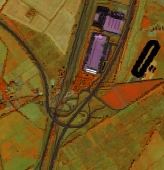
\includegraphics[scale=0.75]{src/seg_input_file.jpg}}
\subfigure[Output for Euclidean distance, $k=70$ and $min\_size=10$]{\label{fig:seg_op_EU}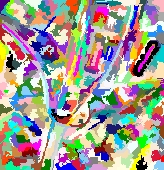
\includegraphics[scale=0.75]{src/seg_output_c70_EU.jpg}}
\subfigure[ Output for SAD, $k=70$ and $min\_size=10$]{\label{fig:seg_op_SAD}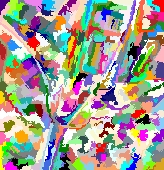
\includegraphics[scale=0.75]{src/seg_output_c70_SAD.jpg}}
\caption{Segmentation output produced by the modified Felzenszwalb and Huttenlocher algorithm}
\end{figure}

\begin{figure}[htbp]
\centering     %%% not \center
\subfigure[Input scene, a sub-region from HyMap02 scene in infrared (bands R=1.0014$\mu m$, G=1.0166 $\mu m$, B=1.0318$\mu m$), with ground truth highroads marked in blue]{\label{fig:gt}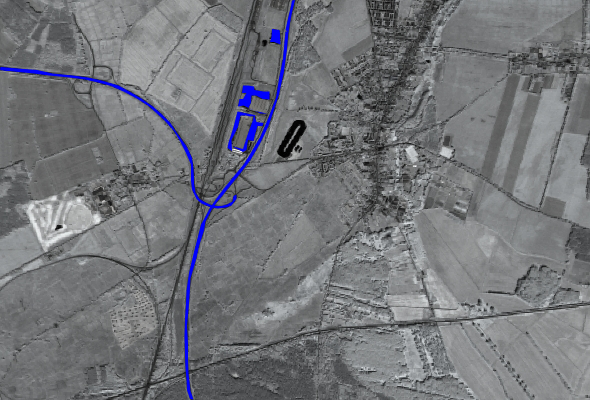
\includegraphics[scale=0.35]{src/gt_hymap02ds02_infra_highroads.jpg}}
\subfigure[ Classified roads for SAD, $k=70$ and $min\_size=10$]{\label{fig:road_op}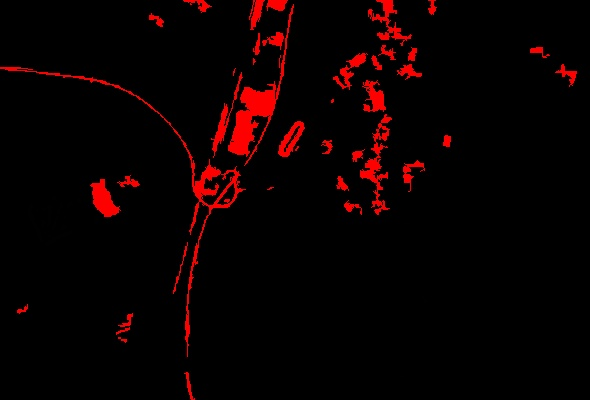
\includegraphics[scale=0.35]{src/op_hymap02ds02_SAD_mean_70_10.jpg}}
\caption{Classification result for approach 1, nearest neighbor mapping using SAD}
\end{figure}

\begin{figure}[hbtp]
\centering
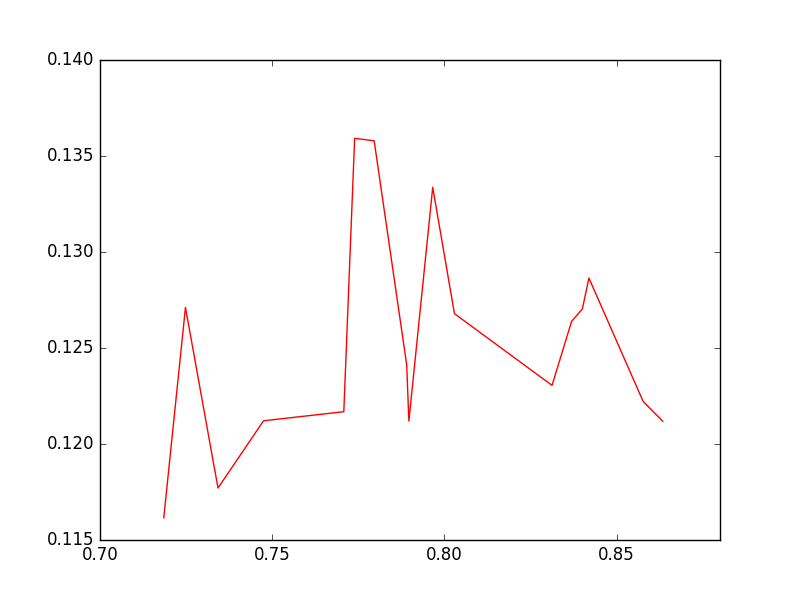
\includegraphics[width=0.75\textwidth]{src/rec_prec_sad.png}
\caption{Recall precision for $min\_size=10$, $k=[10,20,..140]$ }
\label{fig:rec_prec_sad}
\end{figure}

unmixing result very poor.
precision:  0.113970588235
recall:  0.0195214105793
1330 out of 1575 false negative pixels were mapped to spectral 57 (tree10).

\begin{figure}[htbp]
\centering     %%% not \center
\subfigure[Sample false negative pixel spectra, misclassified as Tree 10 ]
{\label{fig:gt}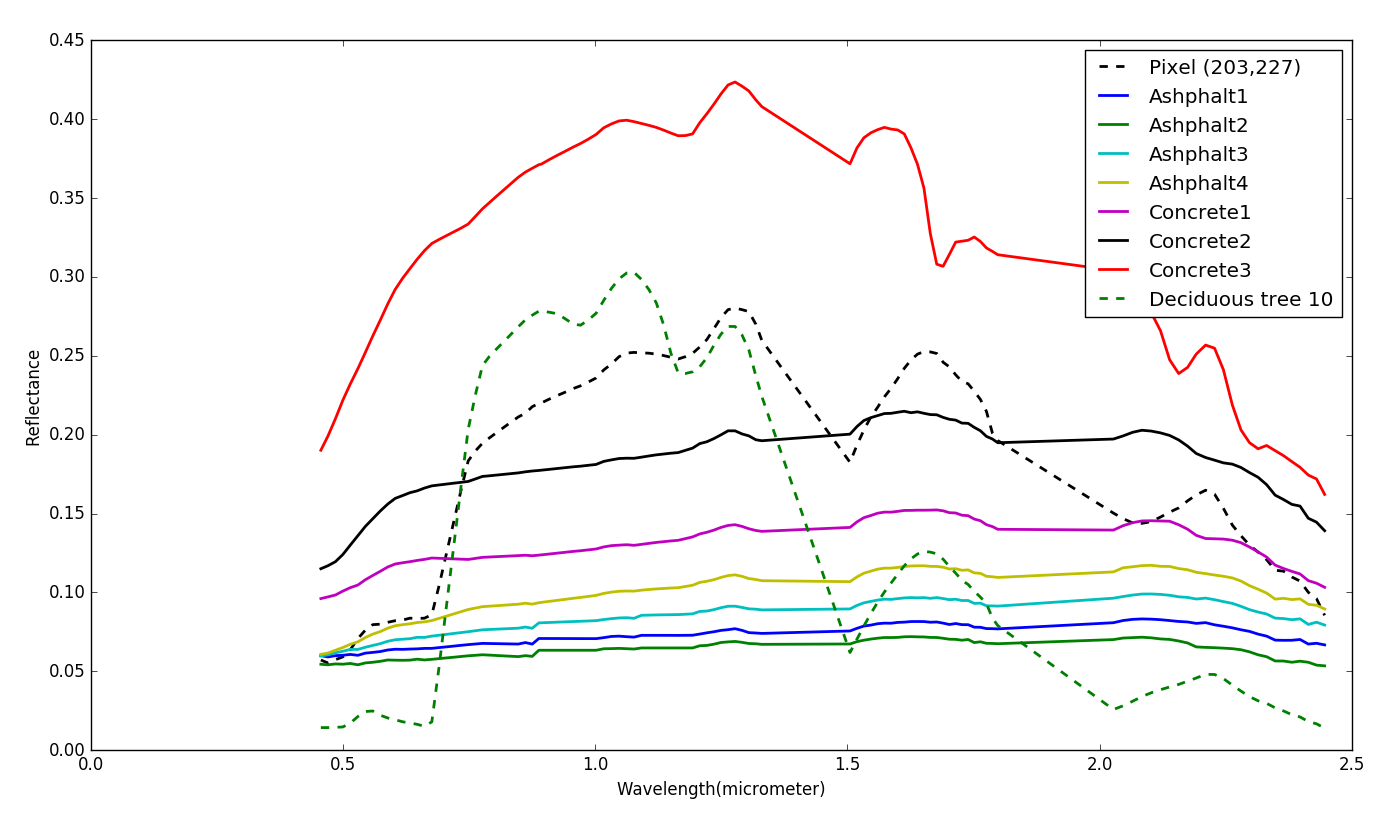
\includegraphics[scale=0.2]{src/px_misclassified_203_277_spectra.png}}
\subfigure[ True Tree 10 pixel spectra ]
{\label{fig:road_op}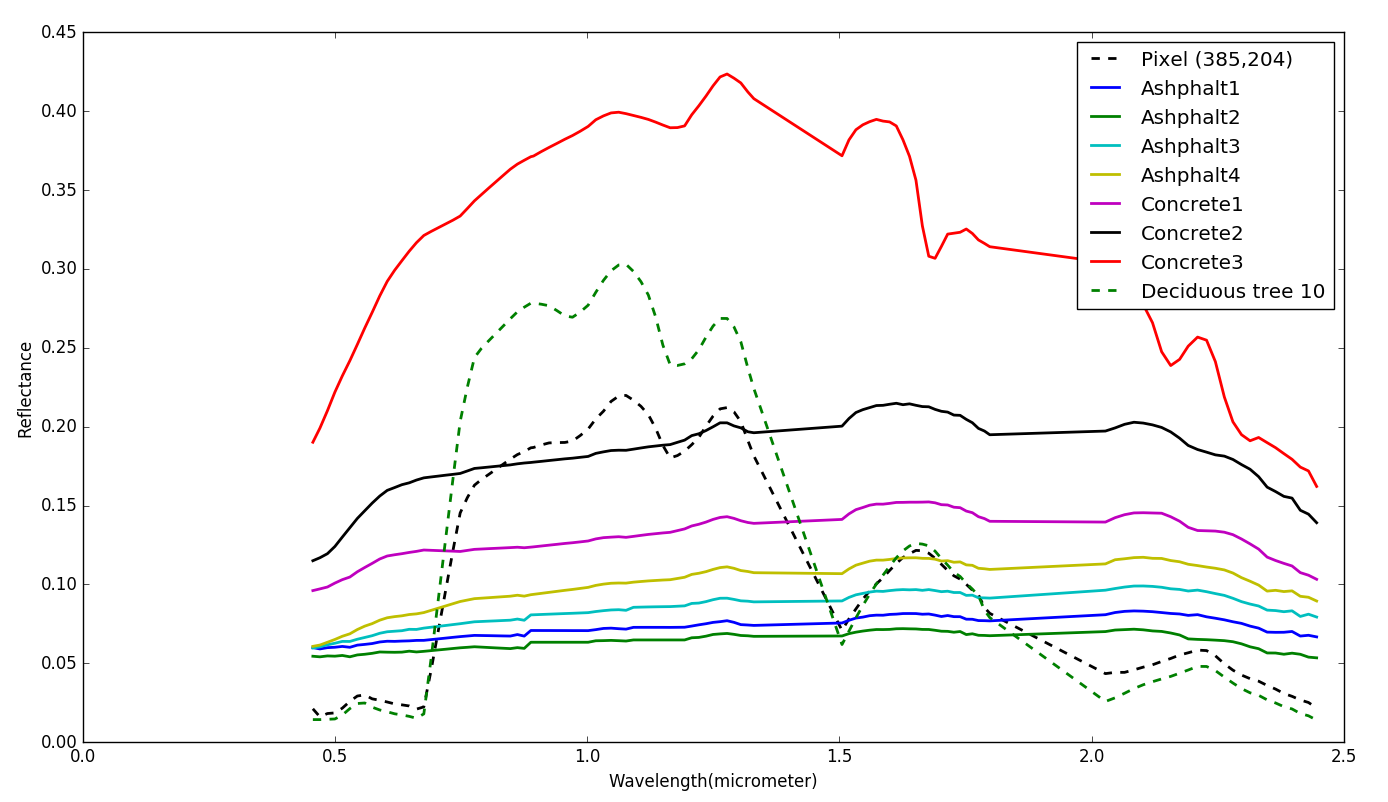
\includegraphics[scale=0.2]{src/px_true_tree57_385_204_spectra.png}}
\caption{Spectral unmixing result analysis}
\end{figure}

\section{Conclusion}
\label{sec:concl}
%%%%%%%%%%%%%%%%%%%%%%%%%%%%%%%%%%%%%%
% hier werden - zum Ende des Textes - die bibliographischen Referenzen
% eingebunden
%
% Insbesondere stehen die eigentlichen Informationen in der Datei
% ``bib.bib''
%
\bibliographystyle{plain}
\bibliography{bib}

\end{document}


